\documentclass[a4paper]{article}

%% Language and font encodings
\usepackage[english]{babel}
\usepackage[utf8x]{inputenc}
\usepackage[T1]{fontenc}

%% Sets page size and margins
\usepackage[a4paper,top=3cm,bottom=2cm,left=3cm,right=3cm,marginparwidth=1.75cm]{geometry}

%% Useful packages
\usepackage{amsmath}
\usepackage{graphicx}
\usepackage{subcaption}
\usepackage[colorinlistoftodos]{todonotes}
\usepackage[colorlinks=true, allcolors=blue]{hyperref}

\title{Actividad 5}
\author{Isaac Neri Gómez Sarmiento}
\date{06 de Marzo, 2018}

\begin{document}
\maketitle


\section{Introducción}
Esta actividad tiene como objetivo el poder ser capaz de limpiar y preparar datos haciendo uso del editor Emacs. Los datos utilizados fueron los de la actividad pasada, especialmente el archivo que concatena el conjunto de datos meteorológicos diarios de todo el año 2017 en la ciudad de Brindisi, Italia. Los valores obtenidos corresponden a la media noche (00z) y medio día (12z) en el meridiano de Greenwich. Para saber la hora correspondiente en Brindisi, solo sumamos una hora. 

\section{Conceptos CAPE y PW}
El acrónimo \textbf{CAPE} se expresa en inglés como \textit{\textbf{Convective Available Potential Energy}} y se traduce como la energía potencial disponible para la convección. Esta magnitud está dada en Joules/Kilogramo y representa la cantidad de energía de empuje disponible para acelerar una parcela de aire verticalmente. También se puede ver como el trabajo realizado por una parcela de aire en el ambiente. 

Esta magnitud ayuda en cierta parte a  detectar zonas en donde la energía potencial es la suficiente como para contribuir a que una tormenta existente se vuelva severa.

El acronimo \textbf{PW} o \textit{\textbf{Precipitable Water}} se traduce en español como Agua Precipitable. Esta magnitud física se mide en milimetros o pulgadas y determina la profundidad del agua de la lluvia que se precita del agua acumulada en forma de gas de una columna en la atmosfera. También sirve como indicador de humedad.



\section{Limpieza y Preparación  de Datos}

Para la limpieza de los datos se utilizó el editor Emacs. Basicamente la información de relleno era seleccionada y remplazada por espacios en blanco o comas. Para el remplazo, se procedió de la siguiente forma:

\begin{enumerate}
\item Seleccionamos uno de los textos repetidos que queremos remplazar con las teclas: \textbf{ctrl + espacio} y la flecha derecha para seleccionar las palabras a subrayar. 

\item Presionamos \textbf{ctrl + w} para cortar y volvemos a colocar el texto mediante \textbf{ctrl +y}

\item Nos ponemos en la parte inicial del archivo con las teclas \textbf{Esc + <}.

\item Volvemos a oprimir \textbf{Esc}, soltamos y presionamos \textbf{\%}

\item Presionamos las teclas \textbf{ctrl +y} y presionamos damos Enter.

\item Se introduce con qué se quiere remplazar el texto seleccionado, presionamos Enter y luego la tecla \textbf{!}.

\item Al hacer los pasos anteriores para la limpieza, obtendremos al final un archivo con los datos de 00Z y 12Z. Finalmente, para separarlos en dos archivos se utilizan el siguiente código que se escribe en la terminal
\begin{verbatim}
$ grep 00Z df2017CAPE_PW.csv > df2017CAPE_PW_00Z.csv
$ grep 12z df2017CAPE_PW.csv > df2017CAPE_PW_12Z.csv
\end{verbatim}
\end{enumerate}

\section{Análisis de datos con Pandas}

Para el análisis de datos se ocuparon las librerias \textbf{pandas}, \textbf{numpy} y \textbf{datetime} en python.

Los pasos que se siguieron para el análisis de datos fueron los siguientes:

\begin{enumerate}
\item Se leyeron los archivos creados y las columna de CAPE se convirtió del tipo objeto a número.

\item La columna de la fecha Date se convirtió de cadena de caracteres a variable temporal "NDate" para adaptar la fecha al formato de lectura que Pandas utiliza: AÑO-MES-DÍA.

\item Se hicieron Boxplots por mes para las magnitudes CAPE y PW para 00z y 12z

\item Se procedió a graficar las magnitudes PW contra CAPE para 00z y 12z con el jointplot de la biblioteca \textbf{seaborn.}



\item Se realizaron 8 gráficas distintias, entre ellas diagramas de caja, de frecuencia, de regresión lineal, etc.

\end{enumerate}

\section{Resultados del análisis}

Las dos gráficas de abajo representan los valores del CAPE de las horas 00Z y 12Z para cada mes.
Podemos ver que en ambas gráficas hay bastantes valores atípicos representados por los puntos grises.
Las medianas de la gráfica de la derecha son ligeramente mayores que las de la izquierda.Esto implica que al mediodia (12z) hay valores más altos de energía potencial disponbile (CAPE).


\begin{figure}[h!]
\centering 
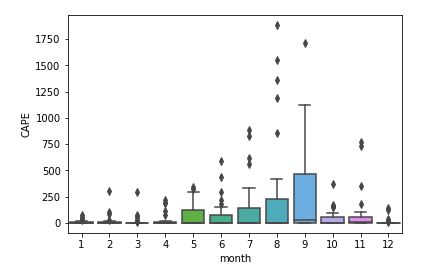
\includegraphics[width=60mm]{Boxplot_CAPE_df00z.JPG}
\label{fig:00Z}
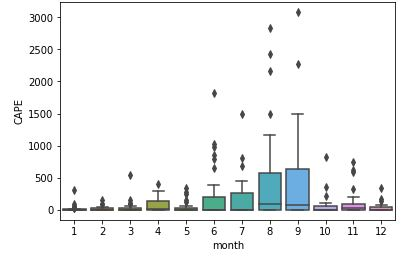
\includegraphics[width=60mm]{Boxplot_CAPE_df12z.JPG}
\label{fig:12Z}   
\caption{Boxplot CAPE para 00Z (izq.) y 12Z (der.)}
\end{figure}



En las gráficas de abajo se representan los valores de PW para 00Z y 12Z. Podemos notar que la gráfica de la izquierda tiene valores atípicos mientras que en la gráfica de la derecha no se presentan ninguno. En los meses de verano, entre mayo y septiembre se puede notar en ambas gráficas que los valores de PW son mayores en comparación con los otros meses, lo cual puede implicar mayor humedad y lluvias.


\begin{figure}[!ht]
\centering 
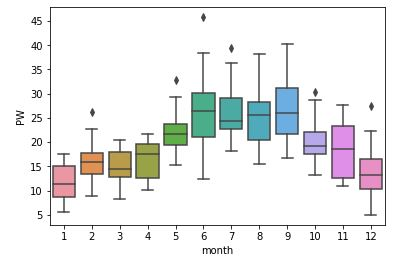
\includegraphics[width=60mm]{Boxplot_PW_df00z.JPG}
%\label{fig:00Z}
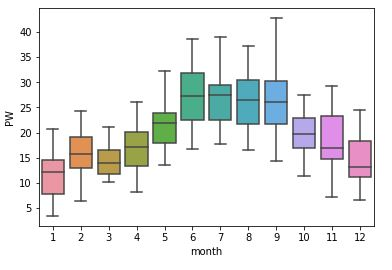
\includegraphics[width=60mm]{Boxplot_PW_df12z.JPG}
%\label{fig:12Z}   
\caption{Boxplot PW para 00Z (izq.) y 12Z (der.)}
\end{figure}


\newpage

Las gráficas de abajo son de PW contra CAPE. En ambas gráficas los meses cuyos colores son más fríos (azul y verde) tienen valores más altos de PW y CAPE. 
No obstante, en ambos casos la mayoria de los puntos están concentrados en el extremo inferior izquierdo.
Podemos ver que para los meses en color rosa, estos tienen muy bajo CAPE Y PW en comparación con otros meses, lo cual implica que las columnas de aire tengan menor energía potencial, teniendo un efecto en la velocidad del viento debido a la disminución de la energía cinética.



\begin{figure}[h!]
\centering 
\includegraphics[width=60mm]{Implot_df00z.JPG}
%\label{fig:00Z}
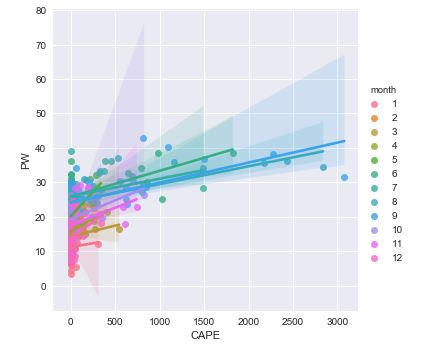
\includegraphics[width=60mm]{Implot_df12z.JPG}
%\label{fig:12Z}   
\caption{Lmplot para 00Z (izq.) y 12Z (der.)}
\end{figure}



Las gráficas de abajo representan la distribución de los datos vertical y horizontalmente de PW contra CAPE. Cada una de las gráficas contiene una recta de regresión lineal, además de mostrar en la parte superior derecha el coeficiente de correlación de Pearson, que indica la correlación lineal entre las dos variables CAPE y PW. Este valor entre más se acerque al cero, ya sea por los negativos o positivos, indica menor relación entre las variables. En este caso, el coeficiente de Pearson de la gráfica de la izquierda es de 0.45, mientras que el de la derecha es de 0.50. Debido a que estos valores son positivos, conforme crece el valor del CAPE, el valor de PW incrementa.





\begin{figure}[h!]
\centering 
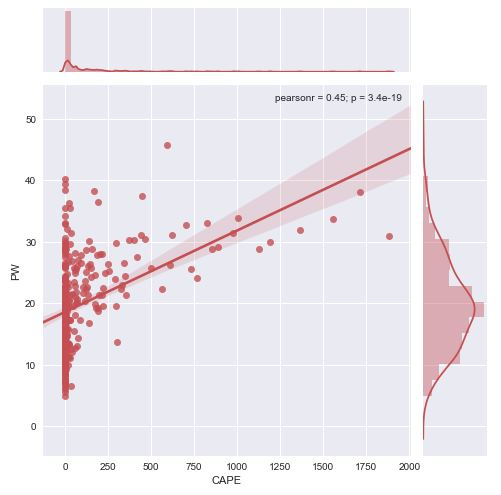
\includegraphics[width=60mm]{Seaborn_joinplot_df00z.JPG}
%\label{fig:00Z}
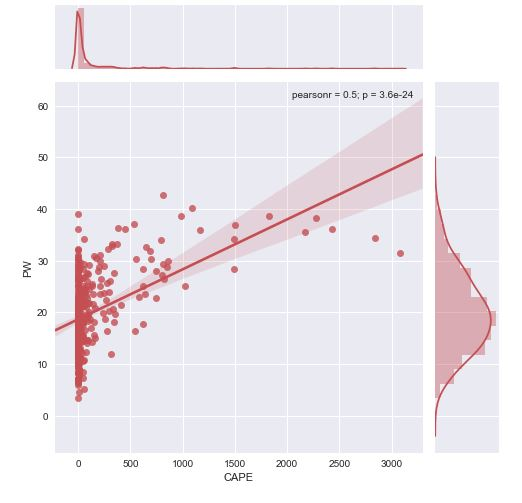
\includegraphics[width=60mm]{Seaborn_joinplot_df12z.JPG}
%\label{fig:12Z}   
\caption{Seaborn joinplot para 00Z (izq.) y 12Z (der.)}
\end{figure}

\newpage

\section{Conclusiones}

Esta práctica más que nada nos sirvió para aprender los comandos básicos para limpiar grandes cantidades de datos para su posterior tabulación y graficación. 

\noindent De las gráficas obtenidas se pudo llegar a la conclusión que los meses que comprende el rango de mayo a septiembre son los más húmedos debido al alto valor del PW comparado con otros meses. Estos meses también tenian valores altos de CAPE, y como ya se había comentado, valores altos de CAPE implican mayor inestabilidad atmosférica y mayor proprensidad a rafagas altas de viento.


\section{Apéndice}
\begin{enumerate}
\item \textbf{¿Cómo se te hizo esta actividad? ¿Compleja, Difícil, Sencilla?}

El nivel de complejidad fue sencillo, solamente en lo que batallé un poco fue en la interpretación de los datos, ya que algunos tipos de gráficas no las había manejado.

\item \textbf{¿Qué te llamó más la atención?}

La forma eficiente de limpiar datos con el uso de Emacs.
\item \textbf{¿Qué parte fue la que menos te interesó hacer?}
Todo fue interesante, no hubo nada que me aburriera o frustara.

\item \textbf{¿Cómo mejorarías esta actividad? ¿Qué le faltó? ¿Qué sobró?}

Tal vez incluyendo más magnitudes físicas para analizar. Estuvo completa la actividad, no estuvo tan saturada de actividades o lecturas como la anterior. 

\item \textbf{¿Hasta este punto, que te parece el uso de Jupyter para programar en Python?}

Me parece una forma más versátil y rápida de visualizar las salidas, como tablas y gráficas en un solo espacio.

\end{enumerate}



\section{Bibliografía}
\begin{itemize}
\item \textit{CAPE.} Tornadochaser. Recuperado el 04/03/2018 de: \url{http://www.tornadochaser.net/cape.html}

\item \textit{Precipitable Water.} Wikipedia. Recuperado el 04/03/2018 de: \url{https://en.wikipedia.org/wiki/Precipitable_water}

\item \textit{Pearsonr.} Scypy. Recuperado el 06/03/2018 de: \url{https://docs.scipy.org/doc/scipy-0.14.0/reference/generated/scipy.stats.pearsonr.html}
\end{itemize}

\end{document}

